\documentclass{standalone}
\usepackage{tikz}
\usetikzlibrary{patterns, positioning}
\usepackage[sfdefault]{ClearSans} %% option 'sfdefault' activates Clear Sans as the default text font
\usepackage[T1]{fontenc}

\begin{document}
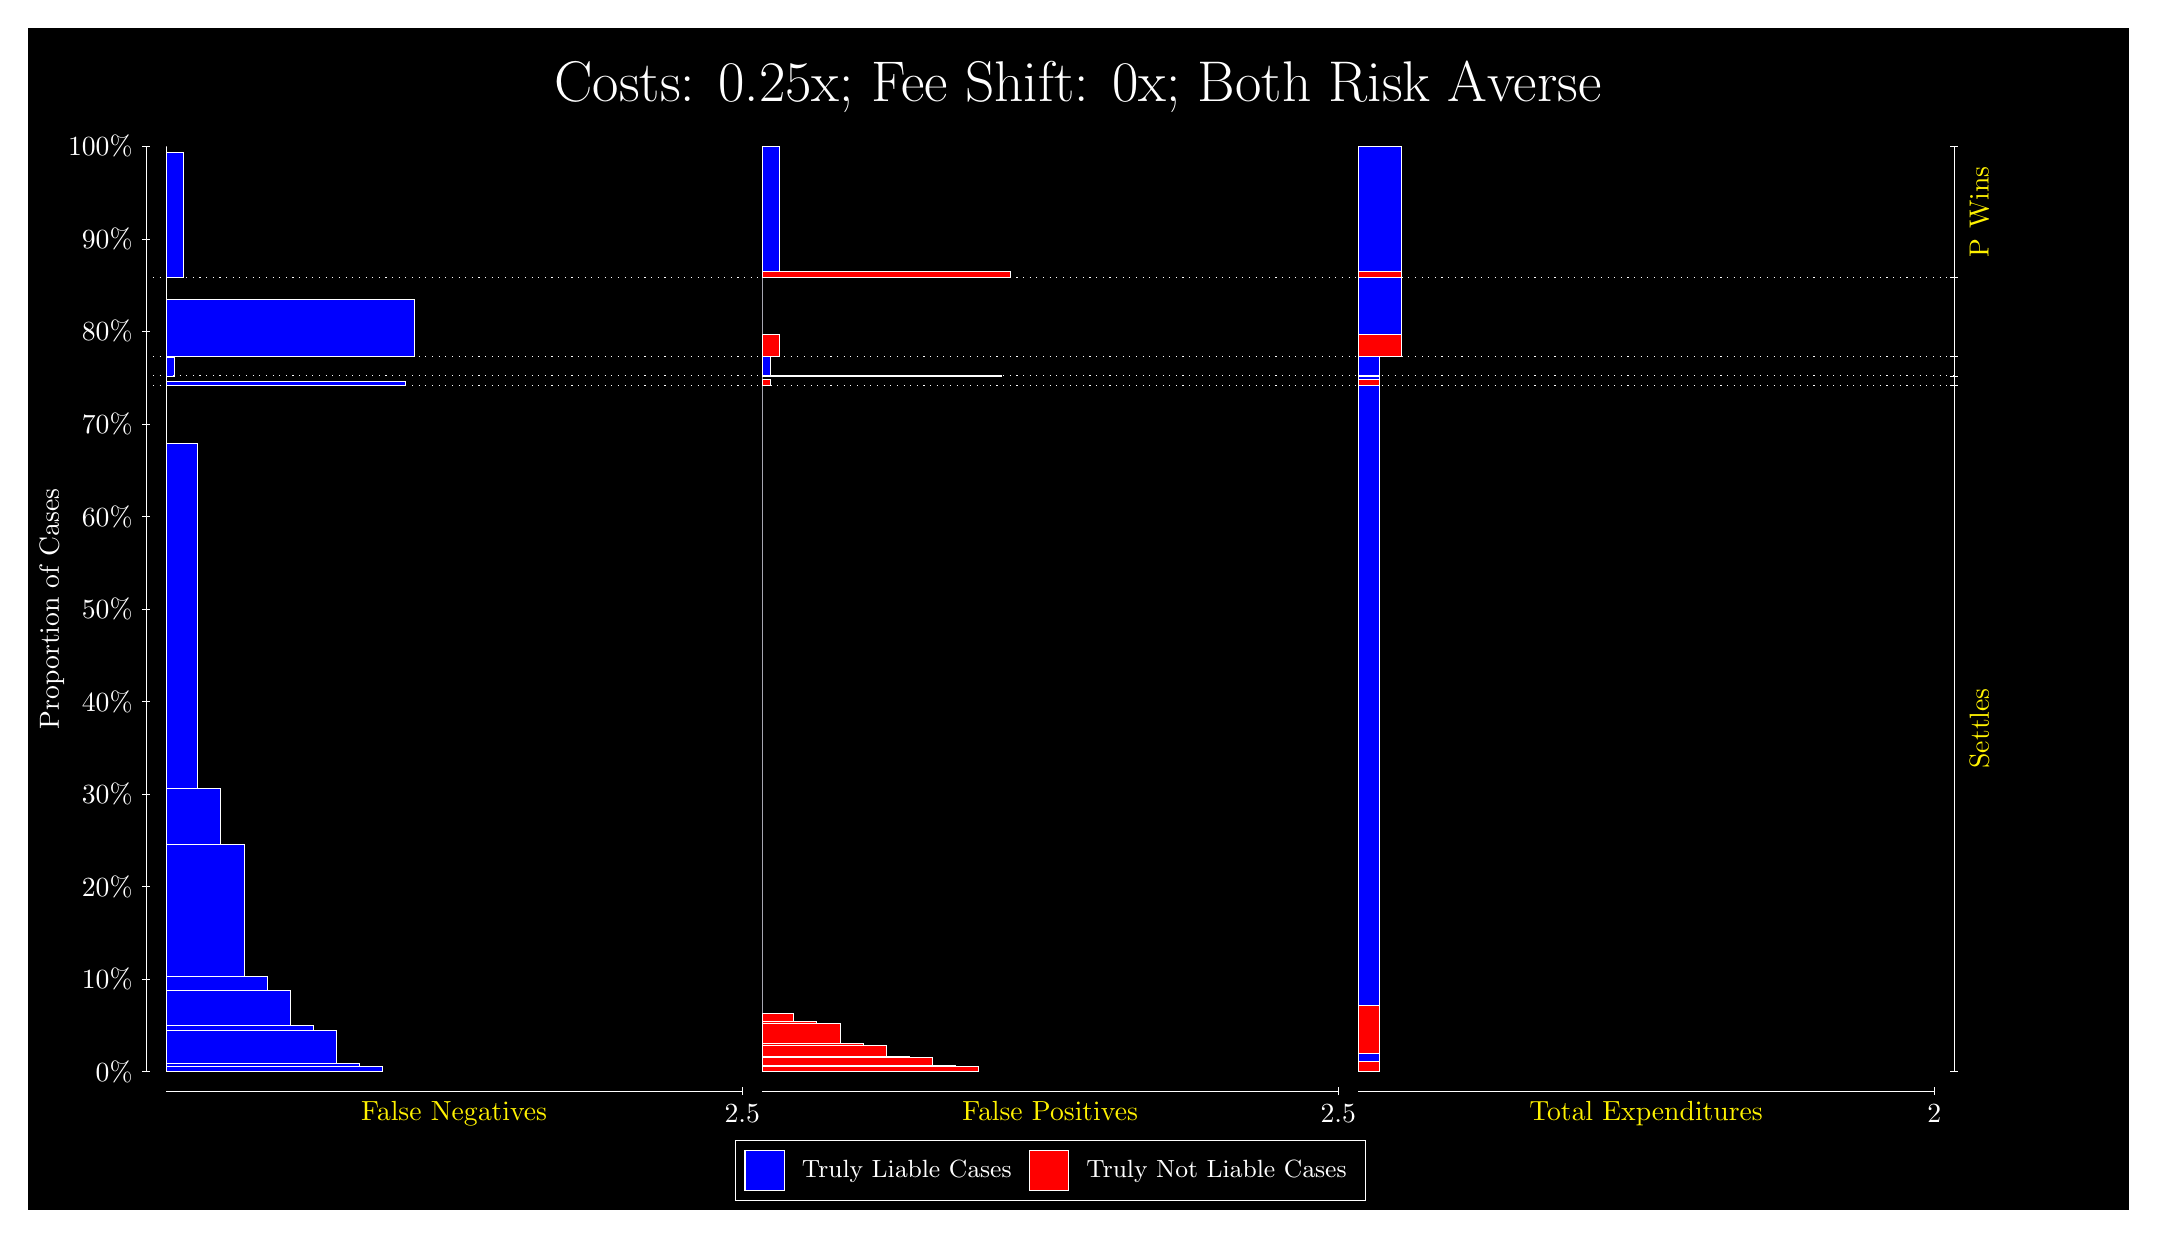
\begin{tikzpicture}
\draw[fill=black] (0,0) rectangle (26.667,15);
\draw[text=white] (0,13.5) rectangle (26.667,15) node[midway] {\huge Costs: 0.25x; Fee Shift: 0x; Both Risk Averse};
\draw[white, very thin] (1.5,1.75) -- (1.5,13.5);
\node[rotate=90, text=white, anchor=center] at (0.3, 7.625) {Proportion of Cases};
\draw[white, very thin] (1.45,1.75) -- (1.55,1.75);
\node[text=white, anchor=east] at (1.45, 1.75) {0\%};
\draw[white, very thin] (1.45,2.925) -- (1.55,2.925);
\node[text=white, anchor=east] at (1.45, 2.925) {10\%};
\draw[white, very thin] (1.45,4.1) -- (1.55,4.1);
\node[text=white, anchor=east] at (1.45, 4.1) {20\%};
\draw[white, very thin] (1.45,5.275) -- (1.55,5.275);
\node[text=white, anchor=east] at (1.45, 5.275) {30\%};
\draw[white, very thin] (1.45,6.45) -- (1.55,6.45);
\node[text=white, anchor=east] at (1.45, 6.45) {40\%};
\draw[white, very thin] (1.45,7.625) -- (1.55,7.625);
\node[text=white, anchor=east] at (1.45, 7.625) {50\%};
\draw[white, very thin] (1.45,8.8) -- (1.55,8.8);
\node[text=white, anchor=east] at (1.45, 8.8) {60\%};
\draw[white, very thin] (1.45,9.975) -- (1.55,9.975);
\node[text=white, anchor=east] at (1.45, 9.975) {70\%};
\draw[white, very thin] (1.45,11.15) -- (1.55,11.15);
\node[text=white, anchor=east] at (1.45, 11.15) {80\%};
\draw[white, very thin] (1.45,12.325) -- (1.55,12.325);
\node[text=white, anchor=east] at (1.45, 12.325) {90\%};
\draw[white, very thin] (1.45,13.5) -- (1.55,13.5);
\node[text=white, anchor=east] at (1.45, 13.5) {100\%};

\draw[white, very thin] (24.457,1.75) -- (24.457,13.5);
\draw[white, very thin] (24.407,1.75) -- (24.507,1.75);
\node[anchor=west] at (24.407, 1.75) {};
\draw[white, very thin] (24.407,10.467) -- (24.507,10.467);
\node[anchor=west] at (24.407, 10.467) {};
\draw[white, very thin] (24.407,10.584) -- (24.507,10.584);
\node[anchor=west] at (24.407, 10.584) {};
\draw[white, very thin] (24.407,10.829) -- (24.507,10.829);
\node[anchor=west] at (24.407, 10.829) {};
\draw[white, very thin] (24.407,11.838) -- (24.507,11.838);
\node[anchor=west] at (24.407, 11.838) {};
\draw[white, very thin] (24.407,13.5) -- (24.507,13.5);
\node[anchor=west] at (24.407, 13.5) {};

\draw[white, very thin, fill=blue] (1.75,1.75) rectangle (4.4946,1.822);
\draw[white, very thin, fill=blue] (1.75,1.822) rectangle (4.2018,1.8495);
\draw[white, very thin, fill=blue] (1.75,1.8495) rectangle (3.9091,2.273);
\draw[white, very thin, fill=blue] (1.75,2.273) rectangle (3.6163,2.3334);
\draw[white, very thin, fill=blue] (1.75,2.3334) rectangle (3.3236,2.7826);
\draw[white, very thin, fill=blue] (1.75,2.7826) rectangle (3.0308,2.9627);
\draw[white, very thin, fill=blue] (1.75,2.9627) rectangle (2.738,4.6314);
\draw[white, very thin, fill=blue] (1.75,4.6314) rectangle (2.4453,5.3484);
\draw[white, very thin, fill=blue] (1.75,5.3484) rectangle (2.1525,9.7277);
\draw[white, very thin, fill=red] (1.75,9.7277) rectangle (1.75,10.467);
\draw[white, very thin, fill=blue] (1.75,10.467) rectangle (4.7873,10.511);
\draw[white, very thin, fill=red] (1.75,10.511) rectangle (1.75,10.584);
\draw[white, very thin, fill=blue] (1.75,10.584) rectangle (1.8598,10.826);
\draw[white, very thin, fill=red] (1.75,10.826) rectangle (1.75,10.829);
\draw[white, very thin, fill=blue] (1.75,10.829) rectangle (4.8971,11.558);
\draw[white, very thin, fill=red] (1.75,11.558) rectangle (1.75,11.838);
\draw[white, very thin, fill=blue] (1.75,11.838) rectangle (1.9696,13.419);
\draw[white, very thin, fill=red] (1.75,13.419) rectangle (1.75,13.5);
\draw[white, very thin, fill=red] (9.3189,1.75) rectangle (12.063,1.8162);
\draw[white, very thin, fill=red] (9.3189,1.8162) rectangle (11.771,1.8279);
\draw[white, very thin, fill=red] (9.3189,1.8279) rectangle (11.478,1.9296);
\draw[white, very thin, fill=red] (9.3189,1.9296) rectangle (11.185,1.9483);
\draw[white, very thin, fill=red] (9.3189,1.9483) rectangle (10.892,2.0783);
\draw[white, very thin, fill=red] (9.3189,2.0783) rectangle (10.6,2.1048);
\draw[white, very thin, fill=red] (9.3189,2.1048) rectangle (10.307,2.36);
\draw[white, very thin, fill=red] (9.3189,2.36) rectangle (10.014,2.3882);
\draw[white, very thin, fill=red] (9.3189,2.3882) rectangle (9.7214,2.4893);
\draw[white, very thin, fill=blue] (9.3189,2.4893) rectangle (9.3189,10.467);
\draw[white, very thin, fill=red] (9.3189,10.467) rectangle (9.4287,10.54);
\draw[white, very thin, fill=blue] (9.3189,10.54) rectangle (9.3189,10.584);
\draw[white, very thin, fill=red] (9.3189,10.584) rectangle (12.356,10.587);
\draw[white, very thin, fill=blue] (9.3189,10.587) rectangle (9.4287,10.829);
\draw[white, very thin, fill=red] (9.3189,10.829) rectangle (9.5384,11.108);
\draw[white, very thin, fill=blue] (9.3189,11.108) rectangle (9.3189,11.838);
\draw[white, very thin, fill=red] (9.3189,11.838) rectangle (12.466,11.918);
\draw[white, very thin, fill=blue] (9.3189,11.918) rectangle (9.5384,13.5);
\draw[white, very thin, fill=red] (16.888,1.75) rectangle (17.162,1.8793);
\draw[white, very thin, fill=blue] (16.888,1.8793) rectangle (17.162,1.9788);
\draw[white, very thin, fill=red] (16.888,1.9788) rectangle (17.162,2.5888);
\draw[white, very thin, fill=blue] (16.888,2.5888) rectangle (17.162,10.467);
\draw[white, very thin, fill=red] (16.888,10.467) rectangle (17.162,10.54);
\draw[white, very thin, fill=blue] (16.888,10.54) rectangle (17.162,10.584);
\draw[white, very thin, fill=red] (16.888,10.584) rectangle (17.162,10.587);
\draw[white, very thin, fill=blue] (16.888,10.587) rectangle (17.162,10.829);
\draw[white, very thin, fill=red] (16.888,10.829) rectangle (17.437,11.108);
\draw[white, very thin, fill=blue] (16.888,11.108) rectangle (17.437,11.838);
\draw[white, very thin, fill=red] (16.888,11.838) rectangle (17.437,11.918);
\draw[white, very thin, fill=blue] (16.888,11.918) rectangle (17.437,13.5);
\draw[white, dotted] (1.5,10.467) -- (24.457,10.467);
\draw[white, dotted] (1.5,10.584) -- (24.457,10.584);
\draw[white, dotted] (1.5,10.829) -- (24.457,10.829);
\draw[white, dotted] (1.5,11.838) -- (24.457,11.838);
\draw[white, very thin] (1.75,1.5) -- (9.0689,1.5);
\node[text=yellow, anchor=north] at (5.4094, 1.5) {False Negatives};
\draw[white, very thin] (9.0689,1.45) -- (9.0689,1.55);
\node[text=white, anchor=north] at (9.0689, 1.45) {2.5};

\draw[white, very thin] (9.3189,1.5) -- (16.638,1.5);
\node[text=yellow, anchor=north] at (12.978, 1.5) {False Positives};
\draw[white, very thin] (16.638,1.45) -- (16.638,1.55);
\node[text=white, anchor=north] at (16.638, 1.45) {2.5};

\draw[white, very thin] (16.888,1.5) -- (24.207,1.5);
\node[text=yellow, anchor=north] at (20.547, 1.5) {Total Expenditures};
\draw[white, very thin] (24.207,1.45) -- (24.207,1.55);
\node[text=white, anchor=north] at (24.207, 1.45) {2};

\node[text=yellow, centered, rotate=90] at (24.777, 6.1085) {Settles};



\node[text=yellow, centered, rotate=90] at (24.777, 12.669) {P Wins};

\draw (12.978300999999998,1.5) node[draw=none] (baseCoordinate) {};
\begin{scope}[align=center]
        \matrix[scale=0.5, draw=white, below=0.5cm of baseCoordinate, nodes={draw}, column sep=0.1cm]{
            \node[rectangle, draw, minimum width=0.5cm, minimum height=0.5cm, fill=blue] {}; &
            \node[draw=none, font=\small, text=white] (B) {Truly Liable Cases}; &
            \node[rectangle, draw, minimum width=0.5cm, minimum height=0.5cm, fill=red] {}; &
            \node[draw=none, font=\small, text=white] (B) {Truly Not Liable Cases}; \\
            };
\end{scope}

\end{tikzpicture}
\end{document}